\documentclass{beamer}
\usepackage[utf8]{inputenc}
\usepackage{graphicx}
\usepackage[justification=centering]{caption}
\usepackage{hyperref}
\usepackage{url}
\usepackage{amsmath}
\usepackage{amssymb}
\usepackage{bm}
\usepackage{pgfplots}

\usepackage{pgfpages}
\setbeameroption{show notes on second screen}

\newcommand{\nth}[1]{$#1^\text{th}$}

\DeclareMathOperator{\sign}{sign}
\DeclareMathOperator{\softmax}{softmax}
\DeclareMathOperator{\loss}{\mathcal{L}}

\usetheme[sectionpage=progressbar, progressbar=frametitle]{metropolis}
\setbeamertemplate{section in toc}{\inserttocsectionnumber.~\inserttocsection}

\title{Fundamentals of Neural Networks}
\date{June 12, 2018}
\author{Mathias Jackermeier}
\institute{Technische Universität München}
\begin{document}
	\maketitle
	\begin{frame}{Introduction}
	\begin{figure}
		\includegraphics[scale=.4]{img/self_driving}
		\caption{A self-driving car. \\Credit: 
			\href{https://www.flickr.com/photos/chijs/21798665468/in/photolist-zdgRMN-HzGNh8-gTzd3u-o5Zrtr-dLznp8-rntpFL-FnbXbs-Hap7Do-9o1FrD-GE5zz3-G9tVGQ-GhD21n-eb2sof-cDdb3y-Gfm7Po-NZGQ3J-GEawvr-FSwEH9-Fnc15o-zhGLV-GbMR1r-FnnkQp-Gfm7CG-eE2tFc-GbMRjx-GbMSe8-9mUNbt-CJdtas}{Marc van der Chijs}
			 / \href{https://creativecommons.org/licenses/by-nd/2.0/}{CC BY-ND 2.0}}
	\end{figure}
	\end{frame}
	\begin{frame}{Introduction}
		\begin{figure}
			\includegraphics[scale=.25]{img/siri}
			\caption{A digital assistant. \\Credit: 
				\href{https://www.flickr.com/photos/65265630@N03/13989720008}{Kārlis Dambrāns} / \href{https://creativecommons.org/licenses/by/2.0/}{CC BY 2.0}}
		\end{figure}
		\note{Jedes intelligente System benutzt neuronale Netze}
	\end{frame}
	\section{The Perceptron}
	\begin{frame}{Example Task}
		\begin{itemize}
			\item<1-> Predict whether an input image of a handwritten digit shows a zero or another digit
		\end{itemize}
	\end{frame}
	\begin{frame}{MNIST Data Sample}
		\begin{figure}
			\includegraphics[scale=1.6]{img/mnist}
			\caption{Examples from the {MNIST} database. \\Credit: 
				\href{https://commons.wikimedia.org/wiki/File:MnistExamples.png}{Josef Steppan}
				/ \href{https://creativecommons.org/licenses/by-sa/4.0/deed.en}{CC BY-SA 4.0}}
		\end{figure}
	\end{frame}
	\begin{frame}{Example Task}
		\begin{itemize}
			\item <1-> Predict whether an input image of a handwritten digit shows a zero or another digit
			\item <1-> The image is represented as a flattened vector of pixel intensities $\bm{x} \in \mathbb{R}^{784}$
			\item <2-> The output should be $1$ if the image shows a zero, otherwise it should be $-1$
			\item <3-> \textbf{Idea}: Assign a weight to every input pixel
		\end{itemize}
	\end{frame}
	\begin{frame}{Model Specification}
		The perceptron accepts $n$ input values and computes an output value $\hat{y}$:
		\begin{equation}
			\begin{split}
			\hat{y} &= \sign\left (\sum_{i=1}^{n} w_ix_i\right )\\
			\equiv \hat{y} &= \sign\left (\bm{w}^\top\bm{x}\right )
			\end{split}
		\end{equation}
	\end{frame}
	\begin{frame}{Visual Representation}
		\begin{figure}
			\input{fig/perceptron_fig}
			\caption{A visual representation of the perceptron model.}
		\end{figure}
		\note{1950\\}
		\note{Neuron im Gehirn: Nervenzelle Eingaben Ausgaben}
	\end{frame}
	\begin{frame}{Generalizations}
		\begin{itemize}
			\item <1-> The perceptron is often used in a modified form
			\item <2-> A scalar bias value can be added to the output computation:
			\begin{equation}
			\hat{y} = \sign\left (\bm{w}^\top\bm{x} + b\right )
			\end{equation}
			\item <3-> The $\sign$ function can be replaced with a generic function $f$:
			\begin{equation}
			\hat{y} = f\left (\bm{w}^\top\bm{x} + b\right )
			\end{equation}
			\item <4-> These modified perceptrons are often called \emph{neurons} or simply \emph{units}
			\item <5-> \textbf{Notation}: We denote the \emph{weighted input} as
			\begin{equation}
			z = \bm{w}^\top\bm{x} + b
			\end{equation}
		\end{itemize}
		\note{f: Aktivierungsfunktion}
	\end{frame}
%	\begin{frame}{Shortcomings of the Perceptron}
%		\begin{figure}
%			% !TeX root = template_Beamer.tex

% restrict y to domain=-1:1, x=1cm
\begin{tikzpicture}[scale=.9]
	\begin{axis}[axis lines = left,xlabel = $x_1$, ylabel = {$x_2$}, ymin=-0.1, ymax=1.1, mlineplot, xmin=-0.1, xmax=1.1]
		\addplot[mark=o,mark size=5pt] coordinates {(0,1)};
		\addplot[mark=o,mark size=5pt] coordinates {(1,0)};
		\addplot[mark=x,mark size=5pt] coordinates {(0,0)};
		\addplot[mark=x,mark size=5pt] coordinates {(1,1)};
	\end{axis}
\end{tikzpicture}			
%			\caption{The perceptron cannot learn the \textsc{xor} function since the data is not linearly separable.}
%		\end{figure}
%	\end{frame}
	
	\section{Feedforward Neural Networks}
	\note{Perzeptron linear: Viele Funktionen können nicht gelernt werden}
	
	\begin{frame}{Networks of neurons}
		\begin{itemize}
			\item <1-> \textbf{Idea}: A combination of multiple neurons could make much better predictions
			\item <2-> A feedforward neural network is a layered architecture of neurons
			\item <3-> The input of a layer is the output of the previous layer
		\end{itemize}
		\note{Angelehnt an Gehirn\\Auch Multilayer Perzeptron}
	\end{frame}
	\begin{frame}{Visual Representation}
		\begin{figure}
			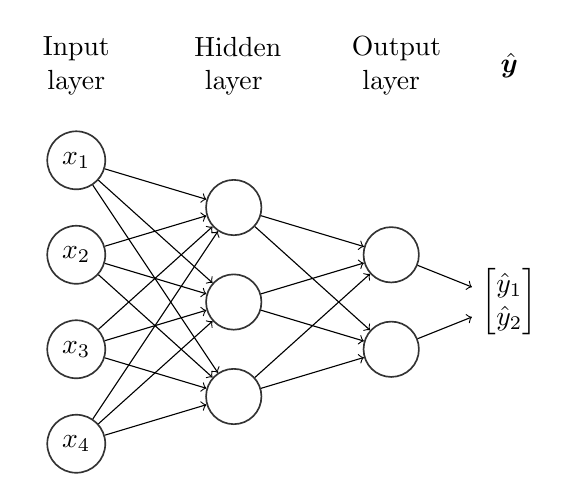
\begin{tikzpicture}
	\tikzstyle{neuron} = [circle,draw=black!80,semithick,minimum size=20pt]
	\tikzstyle{layer} = [text width=1cm, align=center]
	% input layer
	\node[layer] at (0, 0) {Input layer};
	\foreach \i in {1,...,4}
		\node[neuron] (input\i) at (0, -\i*1.2) {$x_\i$};
	% hidden layer
	\node[layer] at (2, 0) {Hidden layer};
	\foreach \i in {1,...,3}
		\node[neuron] (hidden\i) at (2, -\i*1.2 -.6) {};
	% output layer
	\node[layer] at (4, 0) {Output layer};
	\foreach \i in {1,...,2}
		\node[neuron] (output\i) at (4, -\i*1.2 -1.2) {};
	% connections input->hidden
	\foreach \i in {1,...,4}
		\foreach \j in {1,...,3}
			\draw[->] (input\i) -- (hidden\j);
	% connections hidden->output
	\foreach \i in {1,...,3}
		\foreach \j in {1,...,2}
			\draw[->] (hidden\i) -- (output\j);
	
	\node[layer] at (5.5, 0) {$\hat{\bm{y}}$};
	\node (vec) at (5.5, -1.2 - 1.8) {$\begin{bmatrix}\hat{y}_1\\
		\hat{y}_2\end{bmatrix}$};
	\draw[->] (output1) -- (vec);
	\draw[->] (output2) -- (vec);
\end{tikzpicture}
			\caption{A three-layer feedforward neural network.}
		\end{figure}
		\note{Tiefe\\Verbindungen nur zwischen Layers}
	\end{frame}
	\begin{frame}{Output Layer}
		\begin{itemize}
			\item <1-> The design of the output layer depends on the task that we wish to perform
			\item <2-> \emph{Regression}: one single linear neuron
			\item <3-> \emph{Binary classification}: one single sigmoid neuron
		\end{itemize}
	\end{frame}
	\begin{frame}{The Logistic Sigmoid Function}
		\begin{figure}
			\begin{center}
				% !TeX root = template_Beamer.tex

% restrict y to domain=-1:1, x=1cm
\begin{tikzpicture}[scale=.9]
	\begin{axis}[axis lines = left,xlabel = $x$, ylabel = {$\sigma(x)$}, ymin=-0.05, ymax=1.05, mlineplot]
		\addplot [domain=-6:6, samples=200,color=blue, style=semithick]
		{1/(1+exp(-x))};
		%\addlegendentry{$\sigma(x) = 1/\exp(-x)$}
	\end{axis}
\end{tikzpicture}
			\end{center}
			\caption{The logistic sigmoid function $\sigma(x) = \frac1{1+\exp(-x)}$}
			\label{fig:sigmoid}
		\end{figure}
	\end{frame}
	\begin{frame}{Output Layer}
		\begin{itemize}
			\item <1-> The design of the output layer depends on the task that we wish to perform
			\item <1-> \emph{Regression}: one single linear neuron
			\item <1-> \emph{Binary classification}: one single sigmoid neuron
			\item <1-> \emph{Multiclass classification}: $k$ output units with the $\softmax$ function
			\begin{equation}\label{eq:softmax}
			\softmax(x) = \frac{\exp(x)}{\sum_{i=1}^{k}\exp(z_i)}
			\end{equation}
		\end{itemize}
		\note{softmax: Generalisierung, normalisiert\\Viele andere Probleme: Auffälliges Verhalten, Bildgenerierung}
	\end{frame}
	\begin{frame}{Hidden Layers}
		\begin{itemize}
			\item <1-> The task does not give us any information about how to design the hidden layers
			\item <2-> Depth: Irrelevant from a theoretical point of view
			\item <3-> Deep networks perform almost always better in practice
			\item <4-> Activation function: Three common choices are the logistic sigmoid, the $\tanh$, and the rectified linear function
		\end{itemize}
		\note{Daher kommt Deep Learning\\Verschiedene Repräsentationen (Kanten, Objekte,...) $\Rightarrow$ Abstraktionen!\\Kontinuierlich, nicht linear!}
	\end{frame}
	\begin{frame}{The Rectified Linear Function}
		\begin{figure}
			\begin{center}
				% !TeX root = dm-template.tex

% restrict y to domain=-1:1, x=1cm
\begin{tikzpicture}[scale=.9]
	\begin{axis}[axis lines = left,xlabel = $x$, ylabel = {$\max\{0,x\}$}, ymin=-0.5]
		\addplot [domain=-8:8, samples=200, color=blue, style=semithick]
		{max(0,x)};
		%\addlegendentry{$\sigma(x) = 1/\exp(-x)$}
	\end{axis}
\end{tikzpicture}
			\end{center}
			\caption{The rectified linear function $g(x) = \max\{0,x\}$}
			\label{fig:sigmoid}
		\end{figure}
	\end{frame}
	\begin{frame}{Hidden Layers}
		\begin{itemize}
			\item <1-> The task does not give us any information about how to design the hidden layers
			\item <1-> Depth: Irrelevant from a theoretical point of view
			\item <1-> Deep networks perform almost always better in practice
			\item <1-> Activation function: Three common choices are the logistic sigmoid, the $\tanh$, and the rectified linear function
			\item <1-> Experimentation and trial \& error
		\end{itemize}
	\end{frame}
	\begin{frame}{Mathematical Formulation}
		\begin{itemize}
			\item <1-> We can specify a single neuron with a weight vector $\bm{w}$ and a bias value $b$
			\item <2-> Since a neural network consists of multiple neurons in a layer, we need weight \emph{matrices} $\bm{W}^{(l)}$ and bias \emph{vectors} $\bm{b}^{(l)}$ to specify the parameters of a layer $l$
%			\item <3-> The weight $w_{ij}^{(l)}$  is the weight from the \nth{i} neuron in the \nth{(l-1)} layer to the \nth{j} neuron in the \nth{l} layer
%			\item <4-> The bias $b_i^{(l)}$ is the bias of the \nth{i} neuron in the \nth{l} layer
			\item <3-> $f^{(l)}$ is the activation function used in the \nth{l} layer
		\end{itemize}
		\note{f wird komponentenweise angewendet}
	\end{frame}
	\begin{frame}{Mathematical Formulation}
		\begin{itemize}
			\item <1-> The output at layer $l$ is then given by
			\begin{equation}
				\bm{a}^{(l)} = f^{(l)}\left(\bm{W}^{(l)\top}\bm{a}^{(l-1)}+\bm{b}^{(l)}\right)
			\end{equation}
		\end{itemize}
		\note{$a^0 = x$\\$\hat{y} = a^L$}
	\end{frame}
	
	\section{Training Feedforward Neural Networks}
	\begin{frame}{Training Scenario}
		\begin{itemize}
			\item <1-> We have training examples $\mathbb{X} = (\bm{x}^{(1)}, \ldots, \bm{x}^{(m)})$ with corresponding labels $\mathbb{Y}$
			\item <2-> We want to learn a mapping from $\mathbb{X}$ to $\mathbb{Y}$
			\item <3-> \textbf{Idea}: Iteratively adjust the parameters of the neural network
		\end{itemize}
		\note{Zufällig initialisiert}
	\end{frame}
	\begin{frame}{Cost Functions}
		\begin{itemize}
			\item <1-> The cost function $J(\bm{\theta})$ is a measure of how good the network performs
			\item <2-> Learning can be framed as minimizing the cost function
			\item <3-> The total cost is a sum over the costs of the individual training examples:
			\begin{equation}
			J(\bm{\theta}) = \frac1{m}\sum_{i=1}^{m}\loss(\bm{x}^{(i)},\bm{y}^{(i)},\bm{\theta})
			\end{equation}
		\end{itemize}
		\note{Von den Parametern zu einem Skalar\\Größer als 0\\Auch Loss oder Error}
	\end{frame}
	\begin{frame}{Mean squared error}
		\begin{itemize}
			\item <1-> In regression, the per-example loss is commonly
			\begin{equation}
			\loss(\bm{x}, y, \bm{\theta}) = \frac1{2}(\hat{y}-y)^2
			\end{equation}
		\end{itemize}
		\note{Label: Skalar was wir vorhersagen wollen\\Distanz\\Erfüllt Bedingungen}
	\end{frame}
	\begin{frame}{Cross-entropy}
		\begin{itemize}
			\item <1-> In binary classification, we often use the cross-entropy loss
			\begin{equation}
			\loss(\bm{x}, y, \bm{\theta}) = -y \ln \hat{y} - (1-y)\ln(1-\hat{y})
			\end{equation}
		\end{itemize}
		\note{MSE schlecht in Klassifikation\\Label: 1 oder 0}
	\end{frame}
	\begin{frame}{Cross-entropy}
		\begin{itemize}
			\item <1-> In multiclass classification, the cross-entropy becomes
			\begin{equation}
			\loss(\bm{x}, \bm{y}, \bm{\theta}) = -\ln \hat{y}_i
			\end{equation}
		\end{itemize}
		\note{Label: i-te Klasse\\Maximum Likelihood Estimation}
	\end{frame}
	\begin{frame}{Stochastic Gradient Descent}
		\begin{itemize}
			\item <1-> (Stochastic) Gradient Descent is the most common algorithm to minimize cost functions in neural networks
			\item <2-> A change $\Delta \bm{\theta}$ in the parameters corresponds roughly to the change
			\begin{equation}
			\Delta J(\bm{\theta}) \approx \nabla J(\bm{\theta})^{\top}\Delta\bm{\theta}
			\end{equation}
			\item <3-> To minimize $J(\bm{\theta})$, choose
			\begin{equation}
			\Delta\bm{\theta} = -\eta\nabla J(\bm{\theta}),
			\end{equation}
			\item <4-> \emph{Stochastic} Gradient Descent computes only an approximation of the gradient
		\end{itemize}
		\note{$\Rightarrow$ Kleine Änderungen in die entgegengesetze Richtung des Gradienten\\Learning Rate Hyperparameter durch rumexperimentieren\\Erweiterungen}
	\end{frame}
	\begin{frame}{Stochastic Gradient Descent}
		\begin{figure}
			\begin{center}
				\includegraphics[scale=.35]{fig/gradient_descent}
			\end{center}
			\caption{Stochastic Gradient Descent. \\Created with \url{https://academo.org/demos/3d-surface-plotter/}}
		\end{figure}
	\end{frame}
	\begin{frame}{Back-propagation}
		\begin{itemize}
			\item <1-> The back-propagation algorithm efficiently computes the gradient of the cost function
			\item <2-> It can be derived by recursively applying the chain rule to the layers of the neural network, beginning with the output layer
		\end{itemize}
	\end{frame}
	\begin{frame}{Back-propagation}
		\begin{figure}
			\begin{center}
				\tikzset{
	invisible/.style={opacity=0},
	visible on/.style={alt={#1{}{invisible}}},
	alt/.code args={<#1>#2#3}{%
		\alt<#1>{\pgfkeysalso{#2}}{\pgfkeysalso{#3}} % \pgfkeysalso doesn't change the path
	},
}

\begin{tikzpicture}
	\tikzstyle{neuron} = [circle,draw=black!80,semithick,minimum size=20pt]
	\tikzstyle{layer} = [text width=1cm, align=center]
	\tikzstyle{bp} = [->,color=red,thick]
	% input layer
	\node[layer] at (0, 0) {Input layer};
	\foreach \i in {1,...,4}
		\node[neuron] (input\i) at (0, -\i*1.2) {};
	% hidden layer
	\node[layer] at (2, 0) {Hidden layer};
	\foreach \i in {1,...,3}
		\node[neuron] (hidden\i) at (2, -\i*1.2 -.6) {};
	% output layer
	\node[layer] at (4, 0) {Output layer};
	\foreach \i in {1,...,2}
		\node[neuron] (output\i) at (4, -\i*1.2 -1.2) {};
	% connections input->hidden
	\foreach \i in {1,...,4}
		\foreach \j in {1,...,3}
			\draw[->] (input\i) -- (hidden\j);
	% connections hidden->output
	\foreach \i in {1,...,3}
		\foreach \j in {1,...,2}
			\draw[->] (hidden\i) -- (output\j);
	
	\node[layer] at (5.5, 0) {$\hat{\bm{y}}$};
	\node (vec) at (5.5, -1.2 - 1.8) {$\begin{bmatrix}\hat{y}_1\\
		\hat{y}_2\end{bmatrix}$};
	\draw[->] (output1) -- (vec);
	\draw[->] (output2) -- (vec);
	
	\foreach \i in {1,...,4}
		\node[visible on=<1-6>] at (0, -\i*1.2) {$x_\i$};
	
	%backprop
	%frame1
	\foreach \i in {1,...,4}
		\foreach \j in {1,...,3}
			\draw[bp,visible on=<2>] (input\i) -- (hidden\j);
	\foreach \i in {1,...,3}
		\node[visible on=<2-5>] (hidden\i-text) at (2, -\i*1.2 -.6) {$h_\i$};
	%frame2
	\foreach \i in {1,...,3}
		\foreach \j in {1,...,2}
			\draw[bp,visible on=<3>] (hidden\i) -- (output\j);
	\foreach \i in {1,...,2}
		\node[visible on=<3-4>] (hidden\i-text) at (4, -\i*1.2 -1.2) {$o_\i$};
	%frame2
	\draw[bp,visible on=<4>] (output1) -- (vec);
	\draw[bp,visible on=<4>] (output2) -- (vec);
	%frame3
	\draw[bp,visible on=<5>] (vec) -- (output1);
	\draw[bp,visible on=<5>] (vec) -- (output2);
	\foreach \i in {1,...,2}
		\node[visible on=<5->] at (4, -\i*1.2 -1.2) {$\frac{\partial \theta}{\partial J}$};
	%frame4
	\foreach \i in {1,...,2}
		\foreach \j in {1,...,3}
			\draw[bp,visible on=<6>] (output\i) -- (hidden\j);
	\foreach \i in {1,...,3}
		\node[visible on=<6->] at (2, -\i*1.2 -.6) {$\frac{\partial \theta}{\partial J}$};
	%frame5
	\foreach \i in {1,...,3}
		\foreach \j in {1,...,4}
			\draw[bp,visible on=<7>] (hidden\i) -- (input\j);
	\foreach \i in {1,...,4}
		\node[visible on=<7-8>] at (0, -\i*1.2) {$\frac{\partial \theta}{\partial J}$};
\end{tikzpicture}
			\end{center}
			\caption{The Back-propagation algorithm.}
		\end{figure}
	\end{frame}
	\begin{frame}{The Complete Learning Algorithm}
		\begin{enumerate}
			\item <1-> Propagate all training examples of a minibatch forward through the network
			\item <2-> Compute the cost for each training example
			\item <3-> Compute all gradients using back-propagation
			\item <4-> Compute the average gradient
			\item <5-> Update the parameters in the negative direction of the gradient
			\item <6-> Repeat until the cost is low enough
		\end{enumerate}
	\end{frame}
	
	\section{Conclusion}
	\note{Komplexe Netzwerke einfacher Einheiten\\Abstraktionen\\Lernen: Kleine Updates der Parameter so dass das Netzwerk besser wird\\Überall in Deep Learning\\Viele weitere Anwendungen in der Zukunft}
	\begin{frame}[standout]
		Thank you!
	\end{frame}
	
\end{document}